%%%%% Wadler
\begin{frame}
\centering
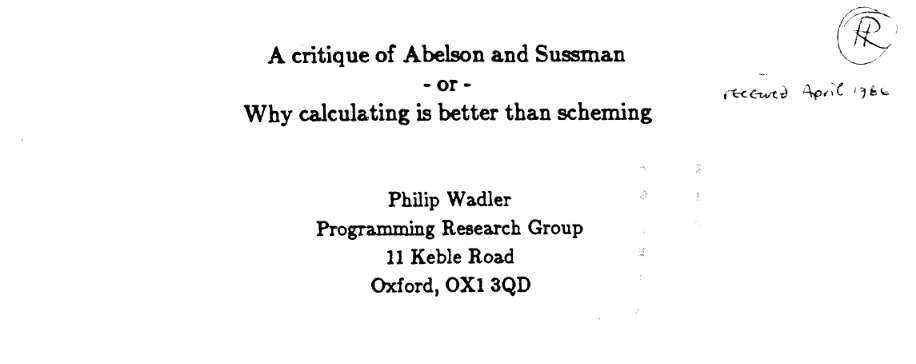
\includegraphics[scale=0.5]{wadler-title.png}
\end{frame}


\begin{frame}
\centering
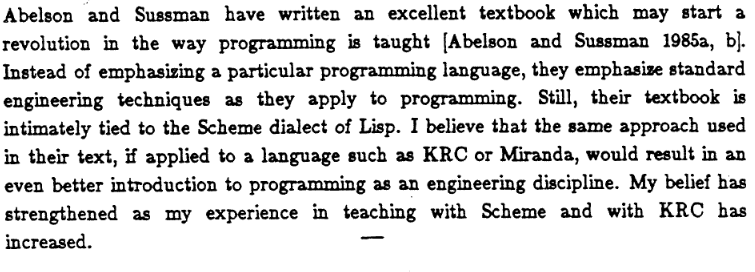
\includegraphics[scale=0.55]{wadler-abstract.png}
% TODO highlight bits?
\end{frame}

\begin{frame}[fragile]
\begin{haskellcode}
perimeter shape =
  case shape of
    Square s      -> s * 4
    Rectangle w h -> 2*w + 2*h
    Circle r      -> 2 * pi * r
\end{haskellcode}
\end{frame}


\begin{frame}[fragile]
\begin{schemecode}
(define (sum items)
  (cond ((null? items) 0)
        (else (+ (car items) (sum (cdr items))))))
\end{schemecode}

\pnl

\begin{haskellcode}
sum items = case items of
  []   -> 0
  x:xs -> x + sum xs
\end{haskellcode}
\end{frame}


\begin{frame}[fragile]
\begin{haskellcode}
[] ++ ys      =  ys
(x:xs) ++ ys  =  x:(xs ++ ys)
\end{haskellcode}

\begin{haskellcode}
(xs ++ ys) ++ zs = xs ++ (ys ++ zs)
\end{haskellcode}
\end{frame}

\iffalse
\begin{frame}[fragile]
\begin{schemecode}
(define (map proc items)
  (if (null? items)
      nil
      (cons (proc (car items))
            (map proc (cdr items)))))
\end{schemecode}
\nl

\begin{haskellcode}
map :: (a -> b) -> [a] -> [b]
map f l =
  case l of
    []       -> []
    (x : xs) -> f x : map f xs
\end{haskellcode}
\end{frame}


\begin{frame}[fragile]
\LARGE
\begin{schemecode}
             (list 3 4)

             (cons 3 4)
\end{schemecode}
\end{frame}


\begin{frame}[fragile]
\begin{columns}[T]
\LARGE
\column{0.5\textwidth}
\begin{schemecode}
  (cons 3 4)
\end{schemecode}

\includegraphics{list-cons1.pdf}

\column{0.5\textwidth}
\begin{schemecode}
  (list 3 4)
\end{schemecode}
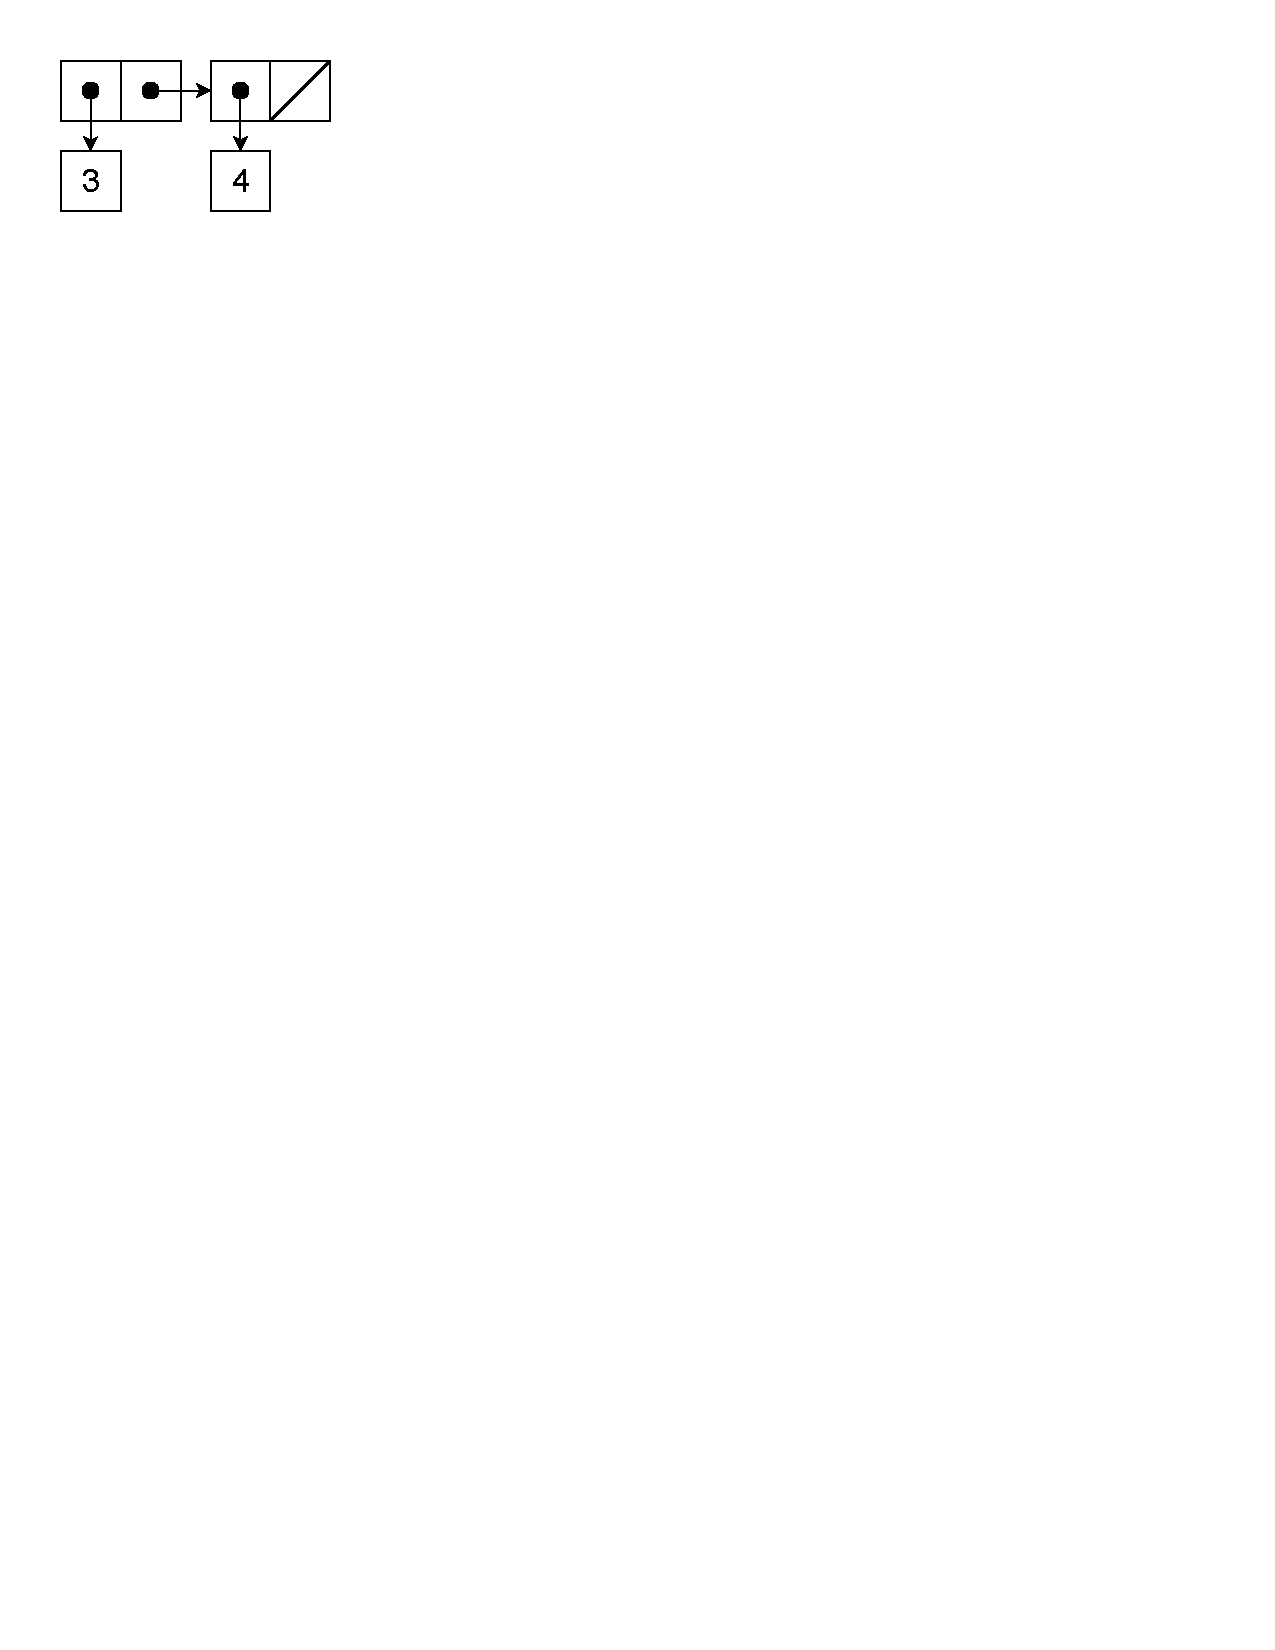
\includegraphics{list-cons2.pdf}
\end{columns}
\end{frame}


\imageslide[0.7]{list-cons-racket.png}
\fi
